\documentclass[11pt, a4paper]{article}\usepackage[]{graphicx}\usepackage[]{color}
%% maxwidth is the original width if it is less than linewidth
%% otherwise use linewidth (to make sure the graphics do not exceed the margin)
\makeatletter
\def\maxwidth{ %
  \ifdim\Gin@nat@width>\linewidth
    \linewidth
  \else
    \Gin@nat@width
  \fi
}
\makeatother

\definecolor{fgcolor}{rgb}{0.345, 0.345, 0.345}
\newcommand{\hlnum}[1]{\textcolor[rgb]{0.686,0.059,0.569}{#1}}%
\newcommand{\hlstr}[1]{\textcolor[rgb]{0.192,0.494,0.8}{#1}}%
\newcommand{\hlcom}[1]{\textcolor[rgb]{0.678,0.584,0.686}{\textit{#1}}}%
\newcommand{\hlopt}[1]{\textcolor[rgb]{0,0,0}{#1}}%
\newcommand{\hlstd}[1]{\textcolor[rgb]{0.345,0.345,0.345}{#1}}%
\newcommand{\hlkwa}[1]{\textcolor[rgb]{0.161,0.373,0.58}{\textbf{#1}}}%
\newcommand{\hlkwb}[1]{\textcolor[rgb]{0.69,0.353,0.396}{#1}}%
\newcommand{\hlkwc}[1]{\textcolor[rgb]{0.333,0.667,0.333}{#1}}%
\newcommand{\hlkwd}[1]{\textcolor[rgb]{0.737,0.353,0.396}{\textbf{#1}}}%

\usepackage{framed}
\makeatletter
\newenvironment{kframe}{%
 \def\at@end@of@kframe{}%
 \ifinner\ifhmode%
  \def\at@end@of@kframe{\end{minipage}}%
  \begin{minipage}{\columnwidth}%
 \fi\fi%
 \def\FrameCommand##1{\hskip\@totalleftmargin \hskip-\fboxsep
 \colorbox{shadecolor}{##1}\hskip-\fboxsep
     % There is no \\@totalrightmargin, so:
     \hskip-\linewidth \hskip-\@totalleftmargin \hskip\columnwidth}%
 \MakeFramed {\advance\hsize-\width
   \@totalleftmargin\z@ \linewidth\hsize
   \@setminipage}}%
 {\par\unskip\endMakeFramed%
 \at@end@of@kframe}
\makeatother

\definecolor{shadecolor}{rgb}{.97, .97, .97}
\definecolor{messagecolor}{rgb}{0, 0, 0}
\definecolor{warningcolor}{rgb}{1, 0, 1}
\definecolor{errorcolor}{rgb}{1, 0, 0}
\newenvironment{knitrout}{}{} % an empty environment to be redefined in TeX

\usepackage{alltt} %or article has only section and below, book and report also have chapter: http://texblog.org/2007/07/09/documentclassbook-report-article-or-letter/

\usepackage[utf8]{inputenc}  % use utf8 encoding of symbols such as umlaute for maximal compatibility across platforms

\usepackage{caption}				% provides commands for handling caption sizes etc.
%\usepackage[a4paper, left=25mm, right=20mm, top=25mm, bottom=20mm]{geometry}		 % to easily change margin widths: https://www.sharelatex.com/learn/Page_size_and_margins



\usepackage{etoolbox}    % for conditional evaluations!
\usepackage[bottom]{footmisc}  % I love footnotes! And they should be down at the bottom of the page!
\usepackage{graphicx}        % when using figures and alike
\usepackage[hidelinks]{hyperref}		% for hyperreferences (links within the document: references, figures, tables, citations)

\usepackage{euler}     % a math font, only for equations and alike; call BEFORE changing the main font; alternatives: mathptmx, fourier, 
%\usepackage{gentium} % for a different font; you can also try: cantarell, charter, libertine, gentium, bera, ... http://tex.stackexchange.com/questions/59403/what-font-packages-are-installed-in-tex-live

%------------------------------------------------------------------------------------------------------
%------- text size settings --------------
\setlength{\textwidth}{16cm}% 
\setlength{\textheight}{25cm} %23 
%(these values were used to fill the page more fully and thus reduce the number of pages!)
\setlength{\topmargin}{-1.5cm} %0
\setlength{\footskip}{1cm} %
%\setlength{\hoffset}{0cm} %
\setlength{\oddsidemargin}{1cm}%
\setlength{\evensidemargin}{-.5cm}%
\setlength{\parskip}{0cm} % Abstand zwischen Absätzen
% ----------------------------------------------------------------
\renewcommand{\textfraction}{0.1} % allows more space to graphics in float
\renewcommand{\topfraction}{0.85}
%\renewcommand{\bottomfraction}{0.65}
\renewcommand{\floatpagefraction}{0.70}


\frenchspacing %http://texwelt.de/wissen/fragen/1154/was-ist-french-spacing-was-macht-frenchspacing



%------------------------------------------------------------------------------------------------------
%------------------------------------------------------------------------------------------------------
\IfFileExists{upquote.sty}{\usepackage{upquote}}{}
\begin{document}
%\SweaveOpts{concordance=TRUE}
%%%%%%%%%%%%% this bit is new to Knitr: %%%%%%%%%%%%%%%%%%%%%



\title{A tutorial for Step Selection Function}

\author{P. Antkowiak\thanks{M.Sc. programme "GIS und Umweltmodellierung" at University of Freiburg} \and H. Tripke\thanks{M.Sc. programme "Wildlife, Biodiversity and Vegetation" at University of Freiburg} \and C. Wilhelm\thanks{M.Sc. programme "Wildlife, Biodiversity and Vegetation" at University of Freiburg}}
% for more control, multiple affiliations, line breaks and alike, use the authblk package!!

\date{\today} % !!use package isodate for more control of date formatting!!

\maketitle

%------------------------------------------------------------------------------------------------------
%------------------------------------------------------------------------------------------------------

\tableofcontents

\newpage

\section{Introduction}%------------------------------------------------------------------------------------------------------
In addition to Resources Selection Functions (RSF) a more detailed anlysis for telemetry data can be conducted by using Step Selection Function (SSF). The use of latter is providing answers to th actual selection of animals on their habitat rather than analysing the use of a habitat only. (DO WE WANT TO CITE, HERE FOR EXAMPLE Simone and friends). So far most of the SSF were done in GIS to use spatial data together with mathematics equations. However, more and more packages are provided in R and thus becomes a valuable alternative. \
This tutorial provides an overview on how to implement SSF with R. The main package we will use in the following is the package \textbf{adehabitatLT}. All single steps that need to be taken care of are summarized in (Figure~\ref{fig:Flowchart}).\
In our tutorial we use telemetry data from Cougars/Mountain Lion (\textit{Latin name}) collected by Simone Ciuti\footnote{we might have to specify that and name and thank the institute.../collected/containing}. As spatial parameters x tables for ruggedness, slope, canopy cover etc. are available. Describe study area...\

\[
\displaystyle w(x) = exp(\beta\1 x1 + \beta\2 x\2 + ... + \beta\px\p)
\]
\
Why did we not use the data (Wildboar) prepared for the adehabitatLT package? - No information on details, metadata provided, it is hard to understand when to use which dataset and why.


\begin{figure} % you can (but shouldn't) use [h] behind {figure} to force the picture to go here. However, the idea of LaTeX is that it will do things for you, so too much interfering is not saving you any time.
% see also here: http://en.wikibooks.org/wiki/LaTeX/Floats,_Figures_and_Captions#Captions
\captionsetup{width=0.8\textwidth}
\centering
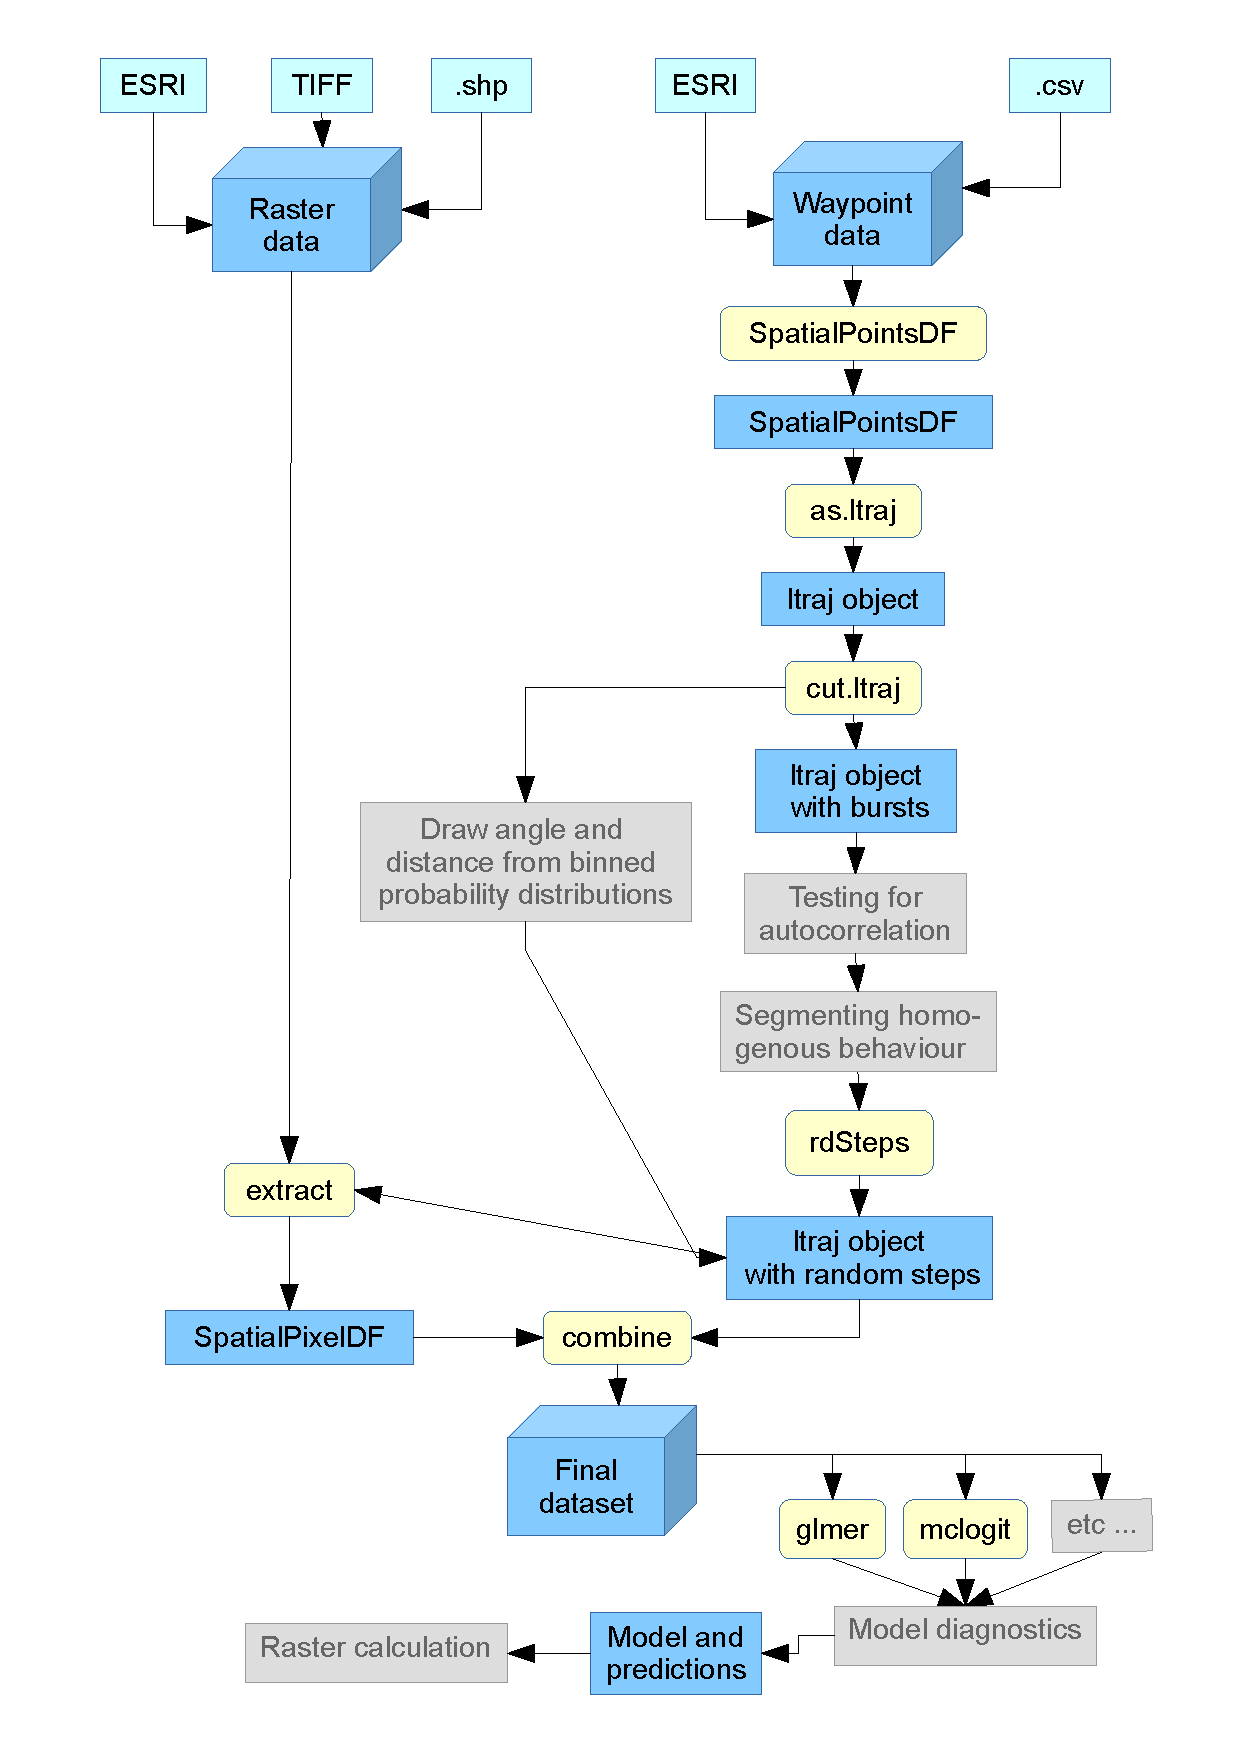
\includegraphics[width=0.8\textwidth]{Flowchart.pdf} %our perfect workflow!
\caption{\emph{Conducting a SSF using existing R-packages:} this figures provides an overview of the steps necessary to conduct a SSF. The steps are separated in subsections, which the turtorial will guide you through.}
\label{fig:Flowchart}
\end{figure}




\section{Preparations}
Before you can actually start using the tutorial for conducting SSF you need to load a bunch of packages in R. Some of them require others so that you have to add all these to your library:

\subsection{Packages - what we need}

\begin{knitrout}
\definecolor{shadecolor}{rgb}{0.969, 0.969, 0.969}\color{fgcolor}\begin{kframe}
\begin{alltt}
\hlcom{# installing packages -----------------------------------------------------}
\hlcom{## for implementing SSF}
\hlcom{# install.packages("adehabitat") # outdated version, not needed for this tutorial}
\hlkwd{install.packages}\hlstd{(}\hlstr{"adehabitatHR"}\hlstd{)}
\hlkwd{install.packages}\hlstd{(}\hlstr{"adehabitatHS"}\hlstd{)}
\hlkwd{install.packages}\hlstd{(}\hlstr{"adehabitatLT"}\hlstd{)}
\hlkwd{install.packages}\hlstd{(}\hlstr{"adehabitatMA"}\hlstd{)}
\hlkwd{install.packages}\hlstd{(}\hlstr{"tkrplot"}\hlstd{)}
\hlkwd{install.packages}\hlstd{(}\hlstr{"hab"}\hlstd{,} \hlkwc{repos} \hlstd{=} \hlstr{"http://ase-research.org/R/"}\hlstd{)} \hlcom{# regular}
\hlkwd{install.packages}\hlstd{(}\hlstr{"hab"}\hlstd{,} \hlkwc{repos} \hlstd{=} \hlstr{"http://ase-research.org/R/"}\hlstd{,} \hlkwc{type} \hlstd{=} \hlstr{"source"}\hlstd{)} \hlcom{# for self-compiling}

\hlcom{# for handling ratser data}
\hlkwd{install.packages}\hlstd{(}\hlstr{"move"}\hlstd{)}
\hlkwd{install.packages}\hlstd{(}\hlstr{"raster"}\hlstd{)}
\hlkwd{install.packages}\hlstd{(}\hlstr{"rgdal"}\hlstd{)}
\hlcom{#install.packages("")}

\hlcom{# loading the packages}
\hlcom{# require(adehabitat) # keep fingers off this package. It is outdated.}
\hlkwd{require}\hlstd{(hab)}
\hlkwd{require}\hlstd{(adehabitatMA)}
\hlkwd{require}\hlstd{(adehabitatHR)}
\hlkwd{require}\hlstd{(adehabitatHS)}
\hlkwd{require}\hlstd{(adehabitatLT)}


\hlcom{## for i dont know}

\hlcom{#require(move)}
\hlcom{#require(raster)}
\hlcom{#require(rgdal)}
\hlcom{#require(tkrplot)}
\hlcom{#require(raster)}
\hlcom{#require(sp)}
\end{alltt}
\end{kframe}
\end{knitrout}



\section{Loading telemetry data (*.csv, ESRI)}%------------------------------------------------------------------------------------------------------

The data for the analysis should be saved in a simple *.csv file format. The table should have column headings in the first line and for each observation include at least the following values: 
\begin{enumerate}
\item{x-coordinate (easting)}
\item{y-coordinate (northing)}
\item{date and/or time}
\item{animal ID}
\end{enumerate}

\noindent Note that the coordinates need to be provided in the same coordinate system and spatial projection as the raster data.

Depending on your analysis you can include further values such as:
\begin{enumerate}
\item{ID for each record}
\item{GPS precision}
\item{other recording parameters such as season}
\item{temperature / elevation at the moment of record}
\item{other values that might be of interest in the further analysis}
\end{enumerate}


\noindent Use the following commands to set your working directory and read the data:
\begin{knitrout}
\definecolor{shadecolor}{rgb}{0.969, 0.969, 0.969}\color{fgcolor}\begin{kframe}
\begin{alltt}
\hlkwd{setwd}\hlstd{(}\hlstr{"/your/working/directory"}\hlstd{)}
\hlstd{xmpl} \hlkwb{=} \hlkwd{read.csv}\hlstd{(}\hlstr{"xmpl.csv"}\hlstd{,} \hlkwc{head}\hlstd{=T)}
\end{alltt}
\end{kframe}
\end{knitrout}

\noindent You can execute \texttt{head(xmpl)} and \texttt{str(xmpl)} to check, whether the data were successfully read.



\section{Creating a Spatial Points Data Frame}%------------------------------------------------------------------------------------------------------
The functions used along the rest of the toolchain can only process data that are stored as objects of class "SpatialPointsDataFrame". This object class stores the coordinates separately and can be created using the according function from package "sp". 

\begin{knitrout}
\definecolor{shadecolor}{rgb}{0.969, 0.969, 0.969}\color{fgcolor}\begin{kframe}
\begin{alltt}
\hlkwd{require}\hlstd{(sp)}

\hlstd{xmpl.spdf} \hlkwb{=} \hlkwd{SpatialPointsDataFrame}\hlstd{(}\hlkwc{coords} \hlstd{= xmpl[,}\hlkwd{c}\hlstd{(}\hlstr{"easting"}\hlstd{,}\hlstr{"northing"}\hlstd{)],} \hlkwc{data} \hlstd{= xmpl)}

\hlkwd{names}\hlstd{(xmpl)}
\end{alltt}
\end{kframe}
\end{knitrout}
In the "coords" argument of the function you should specify the coordinate vectors for your dataset. In our example, we simply assign the two coordinate columns of the example dataset, but you can read the coordinates from a separate file if you want.


\section{Creating an ltraj object}%------------------------------------------------------------------------------------------------------
After storing the data in a Spatial Points Data Frame, you now need to connect the single points and turn them into a set of trajectories. This operation is carried out by the function \texttt{as.ltraj} from the "hab" package and produces objects of class "ltraj".
The function \texttt{as.ltraj} requires at least three arguments to work:
\begin{enumerate}
\item{"xy" (x- and y- coordinates for each point)}
\item{"date" (timestamp for each point, given as POSIXct class)}
\item{"id" (the animal id)}
\end{enumerate}

Both coordinates and animal id can easily be adopted from the Spatial Points Data Frame. The timestamp however, is not stored in the required format yet and you therefore need to convert it first:
\begin{knitrout}
\definecolor{shadecolor}{rgb}{0.969, 0.969, 0.969}\color{fgcolor}\begin{kframe}
\begin{alltt}
\hlstd{date} \hlkwb{<-} \hlkwd{as.POSIXct}\hlstd{(}\hlkwd{strptime}\hlstd{(}\hlkwd{paste}\hlstd{(xmpl.spdf}\hlopt{$}\hlstd{LMT_DATE, xmpl.spdf}\hlopt{$}\hlstd{LMT_TIME),} \hlstr{"%d/%m/%Y  %H:%M:%S"}\hlstd{))}
\end{alltt}
\end{kframe}
\end{knitrout}
It is necessary to combine date and time in one POSIXct value. If your dataset already features a POSIXct timestamp, you can skip this step.

Now you can proceed and actually create the ltraj object by executing the following command:
\begin{knitrout}
\definecolor{shadecolor}{rgb}{0.969, 0.969, 0.969}\color{fgcolor}\begin{kframe}
\begin{alltt}
\hlstd{xmpl.ltr} \hlkwb{<-} \hlstd{hab}\hlopt{:::}\hlkwd{as.ltraj}\hlstd{(}\hlkwc{xy} \hlstd{= xmpl.spdf}\hlopt{@}\hlkwc{coords}\hlstd{,} \hlkwc{date} \hlstd{= date,} \hlkwc{id} \hlstd{= xmpl.spdf}\hlopt{$}\hlstd{cat)}
\end{alltt}
\end{kframe}
\end{knitrout}
Two comments to the function as used: By typing \texttt{hab:::as.ltraj} you tell R to use the \texttt{as.ltraj} function from the "hab" package which is speed optimized against its "adehabitatLT" sibling. Unlike the \texttt{xmpl.spdf@coords} promt which works for any SPDF object, the \texttt{xmpl.spdf$cat} prompt is specific to your dataset. In the example dataset, animal ID's are stored as an integer vector called "cat". If this differs in your dataset and you should change the prompt accordingly.

You now may want to have a closer look at the created ltraj object. Display its structure with by executing \texttt{str(xmpl.ltr)}. 
\begin{knitrout}
\definecolor{shadecolor}{rgb}{0.969, 0.969, 0.969}\color{fgcolor}\begin{kframe}
\begin{alltt}
\hlkwd{str}\hlstd{(xmpl.ltr)}
\end{alltt}
\end{kframe}
\end{knitrout}
When scrolling through the output you will first notice that it consists of 7 elements - the number of individuals in the example dataset. This is because \texttt{as.ltraj()} automatically splits the dataset into subsets one for each individual. We will refine these subsets in the next chapter. Furthermore, the ltraj contains information on the distances and turning angles between consecutive locations.
To get a visual impression of your data you can plot the trajectory for all or for one particular animal:
\begin{knitrout}
\definecolor{shadecolor}{rgb}{0.969, 0.969, 0.969}\color{fgcolor}\begin{kframe}
\begin{alltt}
\hlkwd{plot}\hlstd{(xmpl.ltr)}
\hlkwd{unique}\hlstd{(xmpl.spdf}\hlopt{$}\hlstd{cat)} \hlcom{# prompts a list of all cat ID's. Choose one that you are interested in!}
\hlkwd{plot}\hlstd{(xmpl.ltr,} \hlkwc{id}\hlstd{=}\hlnum{10289}\hlstd{)}
\end{alltt}
\end{kframe}
\end{knitrout}

\section{Creating bursts}


\section{Compute random steps}

The function \textbf{rdSteps} removes the first and the last data point. That's what you want. 



\section{Spatial covariates}%----------------------------------------------------------------------------------------------------------------------------
This section explains the handling of spatial parameters that will be tested for selection by the target species. You should store these data in raster files (ESRI *.adf or georeferenced *.tif). These should have the same coordinate system as your telemetry data and should (for time reasons) already be clipped to your study area and. For instructions how to do this in R, please read the GIS instructions from the other group ;)   

\subsection{Load raster data (ESRI, *.tif, (*.shp))}%------------------------------------------------------------------------------------------------------

With a simple function stored in the package \textbf{raster} you are able to upload any raster file into R. Examplarily we use raster data on the following parameters for the study area:
\begin{enumerate}
\item{ruggedness of the terrain}
\item{land cover}
\item{canopy cover}
\item{distance to the nearest highway}
\item{distance to the nearest road}
\end{enumerate}


\begin{knitrout}
\definecolor{shadecolor}{rgb}{0.969, 0.969, 0.969}\color{fgcolor}\begin{kframe}
\begin{alltt}
\hlkwd{require}\hlstd{(raster)}
\hlkwd{require}\hlstd{(rgdal)}

\hlkwd{require}\hlstd{(sp)}


\hlcom{#?raster}
\hlcom{#getwd()}
\hlcom{#setwd("/home/Peter/")}

\hlstd{ruggedness} \hlkwb{<-} \hlkwd{raster}\hlstd{(}\hlstr{"/home/Peter/Dokumente/uni/WS_14_15/Best Practice R/Dataset/NEW GIS LAYERS/tri1/w001001.adf"}\hlstd{)}
\hlcom{# plot(ruggedness) # outcomment this if you just quickly want to run the script. Takes a minute to process.}

\hlstd{landcover} \hlkwb{<-} \hlkwd{raster}\hlstd{(}\hlstr{"/home/Peter/Dokumente/uni/WS_14_15/Best Practice R/Dataset/NEW GIS LAYERS/lc_30/w001001.adf"}\hlstd{)}
\hlcom{# plot(landcover) # outcomment this if you just quickly want to run the script. Takes a minute to process.}

\hlstd{canopycover} \hlkwb{<-} \hlkwd{raster}\hlstd{(}\hlstr{"/home/Peter/Dokumente/uni/WS_14_15/Best Practice R/Dataset/NEW GIS LAYERS/cc_abmt/w001001.adf"}\hlstd{)}
\hlcom{# plot(canopycover) # outcomment this if you just quickly want to run the script. Takes a minute to process.}

\hlstd{disthighway} \hlkwb{<-} \hlkwd{raster}\hlstd{(}\hlstr{"/home/Peter/Dokumente/uni/WS_14_15/Best Practice R/Dataset/NEW GIS LAYERS/disthwy/w001001.adf"}\hlstd{)}
\hlcom{# plot(disthighway) # outcomment this if you just quickly want to run the script. Takes a minute to process.}

\hlstd{distroad} \hlkwb{<-} \hlkwd{raster}\hlstd{(}\hlstr{"/home/Peter/Dokumente/uni/WS_14_15/Best Practice R/Dataset/NEW GIS LAYERS/distsmrd/w001001.adf"}\hlstd{)}
\hlkwd{plot}\hlstd{(distroad)} \hlcom{# outcomment this if you just quickly want to run the script. Takes a minute to process.}
\end{alltt}
\end{kframe}
\end{knitrout}


\begin{knitrout}
\definecolor{shadecolor}{rgb}{0.969, 0.969, 0.969}\color{fgcolor}\begin{kframe}
\begin{alltt}
\hlcom{# Raster extraction ---------------------------------}

\hlcom{#sp <- SpatialPoints(xy)}
\hlcom{# cougarsRugged <- extract(ruggedness, cougarsSPDF, method='simple', sp=T, df=T) }
\hlcom{# method = 'bilinear' interpolates values from four nearest cells. sp returns Spatial object, df a data frame.}


\hlcom{# first convert the cougars.steps into a SpatialPointsDataFrame}

\hlcom{#cougars.steps.SPDF = SpatialPointsDataFrame(coords = cougars.steps[,c("new_x","new_y")], data = cougars.steps)}
\hlstd{cougars.steps.c.SPDF} \hlkwb{=} \hlkwd{SpatialPointsDataFrame}\hlstd{(}\hlkwc{coords} \hlstd{= cougars.steps.c[,}\hlkwd{c}\hlstd{(}\hlstr{"new_x"}\hlstd{,}\hlstr{"new_y"}\hlstd{)],} \hlkwc{data} \hlstd{= cougars.steps.c)}

\hlcom{#cougars.steps.Rugged <- extract(ruggedness, cougars.steps.SPDF, method='simple', sp=T, df=T) }
\hlcom{#cougars.steps.c.Rugged <- extract(ruggedness, cougars.steps.c.SPDF, method='simple', sp=T, df=T) }

\hlcom{# method = 'simple' extracts value from nearest cell. method = 'bilinear' interpolates from the four nearest cells.}

\hlstd{ruggedness.extr} \hlkwb{<-} \hlkwd{extract}\hlstd{(ruggedness, cougars.steps.c.SPDF,} \hlkwc{method}\hlstd{=}\hlstr{'simple'}\hlstd{,} \hlkwc{sp}\hlstd{=F,} \hlkwc{df}\hlstd{=T)}
\hlstd{landcover.extr} \hlkwb{<-} \hlkwd{extract}\hlstd{(landcover, cougars.steps.c.SPDF,} \hlkwc{method}\hlstd{=}\hlstr{'simple'}\hlstd{,} \hlkwc{sp}\hlstd{=F,} \hlkwc{df}\hlstd{=T)}
\hlstd{canopycover.extr} \hlkwb{<-} \hlkwd{extract}\hlstd{(canopycover, cougars.steps.c.SPDF,} \hlkwc{method}\hlstd{=}\hlstr{'simple'}\hlstd{,} \hlkwc{sp}\hlstd{=F,} \hlkwc{df}\hlstd{=T)}
\hlstd{disthighway.extr} \hlkwb{<-} \hlkwd{extract}\hlstd{(disthighway, cougars.steps.c.SPDF,} \hlkwc{method}\hlstd{=}\hlstr{'simple'}\hlstd{,} \hlkwc{sp}\hlstd{=F,} \hlkwc{df}\hlstd{=T)}
\hlstd{distroad.extr} \hlkwb{<-} \hlkwd{extract}\hlstd{(distroad, cougars.steps.c.SPDF,} \hlkwc{method}\hlstd{=}\hlstr{'simple'}\hlstd{,} \hlkwc{sp}\hlstd{=F,} \hlkwc{df}\hlstd{=T)}





\hlstd{cougars.steps.c.SPDF}\hlopt{$}\hlstd{ruggedness} \hlkwb{<-} \hlstd{ruggedness.extr[,}\hlnum{2}\hlstd{]}
\hlcom{#cougars.steps.c.SPDF$landcover <- landcover.extr[,2]}
\hlstd{cougars.steps.c.SPDF}\hlopt{$}\hlstd{landcover1} \hlkwb{<-} \hlkwd{as.factor}\hlstd{(}
    \hlkwd{ifelse}\hlstd{(landcover.extr[,}\hlnum{2}\hlstd{]} \hlopt{==} \hlnum{0}\hlstd{,}\hlstr{"NA"}\hlstd{,}
    \hlkwd{ifelse}\hlstd{(landcover.extr[,}\hlnum{2}\hlstd{]} \hlopt{<} \hlnum{5}\hlstd{,} \hlstr{"forest"}\hlstd{,}
    \hlkwd{ifelse}\hlstd{(landcover.extr[,}\hlnum{2}\hlstd{]} \hlopt{<} \hlnum{8}\hlstd{,} \hlstr{"open"}\hlstd{,}\hlstr{"NA"}\hlstd{))))}
\hlstd{cougars.steps.c.SPDF}\hlopt{$}\hlstd{canopycover} \hlkwb{<-} \hlstd{canopycover.extr[,}\hlnum{2}\hlstd{]}
\hlstd{cougars.steps.c.SPDF}\hlopt{$}\hlstd{disthighway} \hlkwb{<-} \hlstd{disthighway.extr[,}\hlnum{2}\hlstd{]}
\hlstd{cougars.steps.c.SPDF}\hlopt{$}\hlstd{distroad} \hlkwb{<-} \hlstd{distroad.extr[,}\hlnum{2}\hlstd{]}


\hlkwd{head}\hlstd{(cougars.steps.c.SPDF)}

\hlcom{#head(cougars.steps.Rugged)}
\hlcom{#View(cougars.steps.Rugged)}

\hlcom{#head(cougars.steps.c.Rugged)}
\hlcom{#View(cougars.steps.c.Rugged)}


\hlcom{#names(ruggedness)}
\hlcom{#head(cougars)}
\hlcom{#head(cougarsRugged)}
\end{alltt}
\end{kframe}
\end{knitrout}




\subsection{Extract coordinates for comparison of used and random points} %------------------------------------------------------------------------------------------------------
Peter is successfully doing this step!!

\section{Final SSF model}


\section{Acknowledgements}
Don't forget to thank TeX and R and other opensource communities if you use their products! The correct way to cite R is shown when typing ``\texttt{citation()}'', and ``\texttt{citation("mgcv")}'' for packages.



\end{document}
